% Options for packages loaded elsewhere
\PassOptionsToPackage{unicode}{hyperref}
\PassOptionsToPackage{hyphens}{url}
%
\documentclass[
]{article}
\usepackage{amsmath,amssymb}
\usepackage{lmodern}
\usepackage{iftex}
\ifPDFTeX
  \usepackage[T1]{fontenc}
  \usepackage[utf8]{inputenc}
  \usepackage{textcomp} % provide euro and other symbols
\else % if luatex or xetex
  \usepackage{unicode-math}
  \defaultfontfeatures{Scale=MatchLowercase}
  \defaultfontfeatures[\rmfamily]{Ligatures=TeX,Scale=1}
\fi
% Use upquote if available, for straight quotes in verbatim environments
\IfFileExists{upquote.sty}{\usepackage{upquote}}{}
\IfFileExists{microtype.sty}{% use microtype if available
  \usepackage[]{microtype}
  \UseMicrotypeSet[protrusion]{basicmath} % disable protrusion for tt fonts
}{}
\makeatletter
\@ifundefined{KOMAClassName}{% if non-KOMA class
  \IfFileExists{parskip.sty}{%
    \usepackage{parskip}
  }{% else
    \setlength{\parindent}{0pt}
    \setlength{\parskip}{6pt plus 2pt minus 1pt}}
}{% if KOMA class
  \KOMAoptions{parskip=half}}
\makeatother
\usepackage{xcolor}
\usepackage[margin=1in]{geometry}
\usepackage{graphicx}
\makeatletter
\def\maxwidth{\ifdim\Gin@nat@width>\linewidth\linewidth\else\Gin@nat@width\fi}
\def\maxheight{\ifdim\Gin@nat@height>\textheight\textheight\else\Gin@nat@height\fi}
\makeatother
% Scale images if necessary, so that they will not overflow the page
% margins by default, and it is still possible to overwrite the defaults
% using explicit options in \includegraphics[width, height, ...]{}
\setkeys{Gin}{width=\maxwidth,height=\maxheight,keepaspectratio}
% Set default figure placement to htbp
\makeatletter
\def\fps@figure{htbp}
\makeatother
\setlength{\emergencystretch}{3em} % prevent overfull lines
\providecommand{\tightlist}{%
  \setlength{\itemsep}{0pt}\setlength{\parskip}{0pt}}
\setcounter{secnumdepth}{-\maxdimen} % remove section numbering
\usepackage{titling} \pretitle{\begin{center} \vspace{-2cm}
\includegraphics[width=\linewidth,height=0.7in]{images/Base_info/logo.png}\LARGE\\} \posttitle{\end{center}} \usepackage{float} \usepackage{fancyhdr} \usepackage{ragged2e} \usepackage{caption} \captionsetup[figure]{labelformat=empty} \pagestyle{fancy} \fancyhead[L,C]{} \fancypagestyle{plain}{\pagestyle{fancy}}
\usepackage{booktabs}
\usepackage{longtable}
\usepackage{array}
\usepackage{multirow}
\usepackage{wrapfig}
\usepackage{float}
\usepackage{colortbl}
\usepackage{pdflscape}
\usepackage{tabu}
\usepackage{threeparttable}
\usepackage{threeparttablex}
\usepackage[normalem]{ulem}
\usepackage{makecell}
\usepackage{xcolor}
\ifLuaTeX
  \usepackage{selnolig}  % disable illegal ligatures
\fi
\IfFileExists{bookmark.sty}{\usepackage{bookmark}}{\usepackage{hyperref}}
\IfFileExists{xurl.sty}{\usepackage{xurl}}{} % add URL line breaks if available
\urlstyle{same} % disable monospaced font for URLs
\hypersetup{
  pdftitle={Blastocerus dichotomus},
  hidelinks,
  pdfcreator={LaTeX via pandoc}}

\title{\emph{Blastocerus dichotomus}}
\usepackage{etoolbox}
\makeatletter
\providecommand{\subtitle}[1]{% add subtitle to \maketitle
  \apptocmd{\@title}{\par {\large #1 \par}}{}{}
}
\makeatother
\subtitle{\textbf{Ciervo de los pantanos}}
\author{}
\date{\vspace{-2.5em}Fecha de creación: 29 marzo, 2023}

\begin{document}
\maketitle

\fancyhead[R]{\textbf{doi:https://d.1025CMAoideprueba}}

\center

\hypertarget{autores-pereira-javier-a.-varela-diego-aprile-gustavo-cirignoli-sebastiuxe1n-orozco-maruxeda-marcela-lartigau-bernardo-de-angelo-carlos-giraudo-alejandro-r.}{%
\subsection{\texorpdfstring{\textbf{Autores: Pereira, Javier A.; Varela,
Diego; Aprile, Gustavo; Cirignoli, Sebastián; Orozco, María Marcela;
Lartigau, Bernardo; De Angelo, Carlos; Giraudo, Alejandro
R.}}{Autores: Pereira, Javier A.; Varela, Diego; Aprile, Gustavo; Cirignoli, Sebastián; Orozco, María Marcela; Lartigau, Bernardo; De Angelo, Carlos; Giraudo, Alejandro R.}}\label{autores-pereira-javier-a.-varela-diego-aprile-gustavo-cirignoli-sebastiuxe1n-orozco-maruxeda-marcela-lartigau-bernardo-de-angelo-carlos-giraudo-alejandro-r.}}

\begin{center}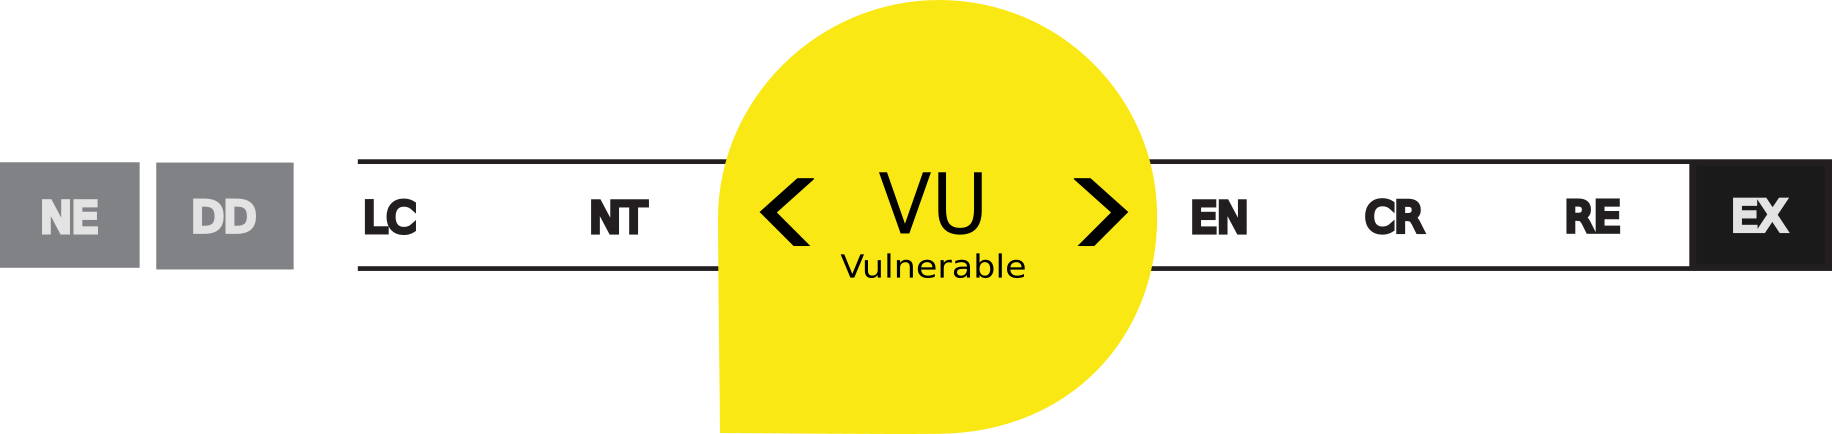
\includegraphics[width=0.7\linewidth]{images/scale-vu} \end{center}

\begin{center}
\includegraphics[width=0.7\linewidth]{images/cma-logo} \end{center}

\begin{center}\rule{0.5\linewidth}{0.5pt}\end{center}

\justifying

\textbf{Citar como:} Pereira, Javier A.; Varela, Diego; Aprile, Gustavo;
Cirignoli, Sebastián; Orozco, María Marcela; Lartigau, Bernardo; De
Angelo, Carlos; Giraudo, Alejandro R.. (2019). \emph{Blastocerus
dichotomus}. En: SAyDS--SAREM (eds.) Categorización 2019 de los
mamíferos de Argentina según su riesgo de extinción. Lista Roja de los
mamíferos de Argentina. Versión digital: \url{http://cma.sarem.org.ar}.

\begin{center}\rule{0.5\linewidth}{0.5pt}\end{center}

\newpage

\begin{figure}[H]

{\centering 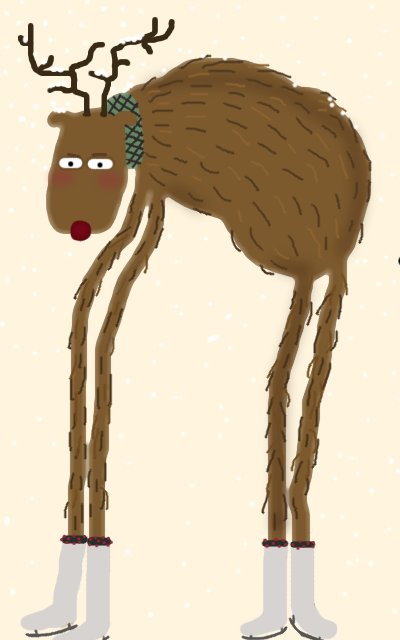
\includegraphics[width=0.5\linewidth]{photos/Blastocerus dichotomus} 

}

\caption{Fotos por Salvador Dali}\label{fig:image}
\end{figure}

\textbf{Categoría Nacional de Conservación 2019}

VU (Vulnerable)

\textbf{Criterios y subcriterios}

A3cde

\textbf{Justificación de la categorización}

El ciervo de los pantanos es una especie dependiente de ambientes de
humedales y está sujeto a una alta presión de caza furtiva. Su rango de
distribución se encuentra fragmentado en al menos cuatro subpoblaciones.
Si bien la subpoblación de los Esteros del Iberá y áreas adyacentes, en
la provincia de Corrientes, ha experimentado una importante recuperación
en los últimos 30 años, el resto de las subpoblaciones se encuentran
amenazadas (ver Evaluación de Subpoblaciones). La caza furtiva y el
drenaje de los humedales para la producción agropecuaria, forestaciones
y urbanizaciones son sus principales amenazas. La especie se ve afectada
por las inundaciones extraordinarias que provocan mortalidades masivas
por aumento en la presión de cacería, desnutrición, enfermedades y
temperaturas extremas. Algunas subpoblaciones también se encuentran
amenazadas por el ataque de perros, la competencia por interferencia con
el ganado bovino y el atropellamiento en rutas. A nivel nacional, la
especie está categorizada como Vulnerable (VU) con una proyección de
reducción de su tamaño poblacional del 30\% hacia el futuro (15 años,
tres generaciones), teniendo en cuenta la reducción del EOO, AOO y la
calidad de hábitat, y los impactos de la caza furtiva y de las
inundaciones extraordinarias (incrementadas por el cambio climático).

\end{document}
